\documentclass{article}

% Images
\usepackage{float}
\usepackage{graphicx}
\usepackage{subcaption}

% Item Enumeration
\usepackage{enumitem}
% Easy List
\usepackage[ampersand]{easylist}

% References
\usepackage{hyperref}

\title{Identificación y Control Neuronal}

\author{Pablo Acereda //
        Laura Pérez}

\begin{document}

% Title
\maketitle

% This page has been left blank intentionally
\newpage
\vspace*{\fill}
 \begin{center}
This page has been intentionally left blank
 \end{center}
\vspace*{\fill}
\newpage

% Table of contents
\tableofcontents

\newpage

\section{Ejercicio 1. Perceptron}

\section{Ejercicio 2. Aproximación de funciones}

En todos los casos, y con los diferentes métodos de entrenamiento, el
incrementar el tamaño de la capa oculta implica una mayor precisión, número de
iteraciones para completar el proceso y un pequeño incremento del tiempo de
procesado.

En cuanto a las funciones de entrenamiento, se han empleado:

\begin{description}
\item [trainbr] Bayesan Regularization
\item [trainrp] Resilient Backpropagation
\item [trainoss] One Step Secant
\item [traingd] Gradient Descent
\end{description}

\begin{figure}[h]
 \centering
 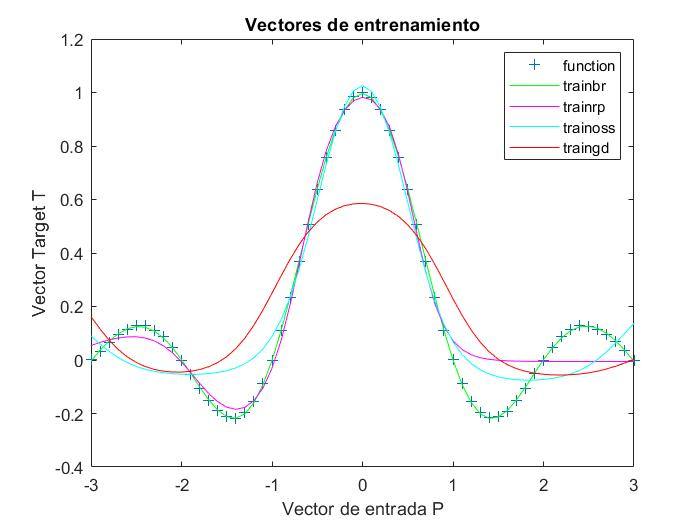
\includegraphics[width=0.8\textwidth]{../I_ex2/training_functions.jpg}
 \caption{Funciones de entrenamiento empleadas.} 
 \label{tf}
\end{figure}

Cambiar la función de entrenamiento puede dar resultados completamente
diferentes. Como se observa en \hyperref[tf]{\ref{tf}} emplear diferentes
funciones puede afectar al tiempo de entrenamiento; al número de iteraciones
(siendo en este caso \textit{traingd} la más costosa); y a la precisión de los
valores obtenidos (siendo \textit{trainbr} la más precisa).

\end{document}
